\section{Simulation Results}
The simulation results presented in Fig.’s \ref{fig:2D_Plot_4Tractor_MB} and \ref{fig:Traj_4Tractor_MB} for the multi-body system show four tractors attempting to navigate $\sim$15m of a soft, low traction terrain denoted as Terrain 2. One tractor (black) takes no action with the winch and becomes immobilized while three others (red, blue, green) use different sets of open loop control inputs to maintain mobility. Plots for $X_T$, $v_T$, $\psi r_W$, $\dot\psi r_W$, and $v_{SD}$ are shown in Fig. \ref{fig:Traj_4Tractor_MB}. The blue vehicle maintains a very low braking pressure that minimizes drawbar pull and maximizes vehicle speed. However, the loss of cable length along the soft terrain for this vehicle is also the highest among all vehicles. The green vehicle pulse brakes and loses $\sim$3.5m less in cable than the blue vehicle but has large fluctuations in its speed. After the tractors navigate Terrain 2, the towed load is pulled back in. The open loop responses can be seen in Figure 6 from $\sim$24-30 seconds and show how the red and blue tractors have more stable responses when compared to the green one. This is caused by the limitations of the pressure compensation for the variable displacement pump when $P_{set}$
\begin{figure}[hb]
    \centering
    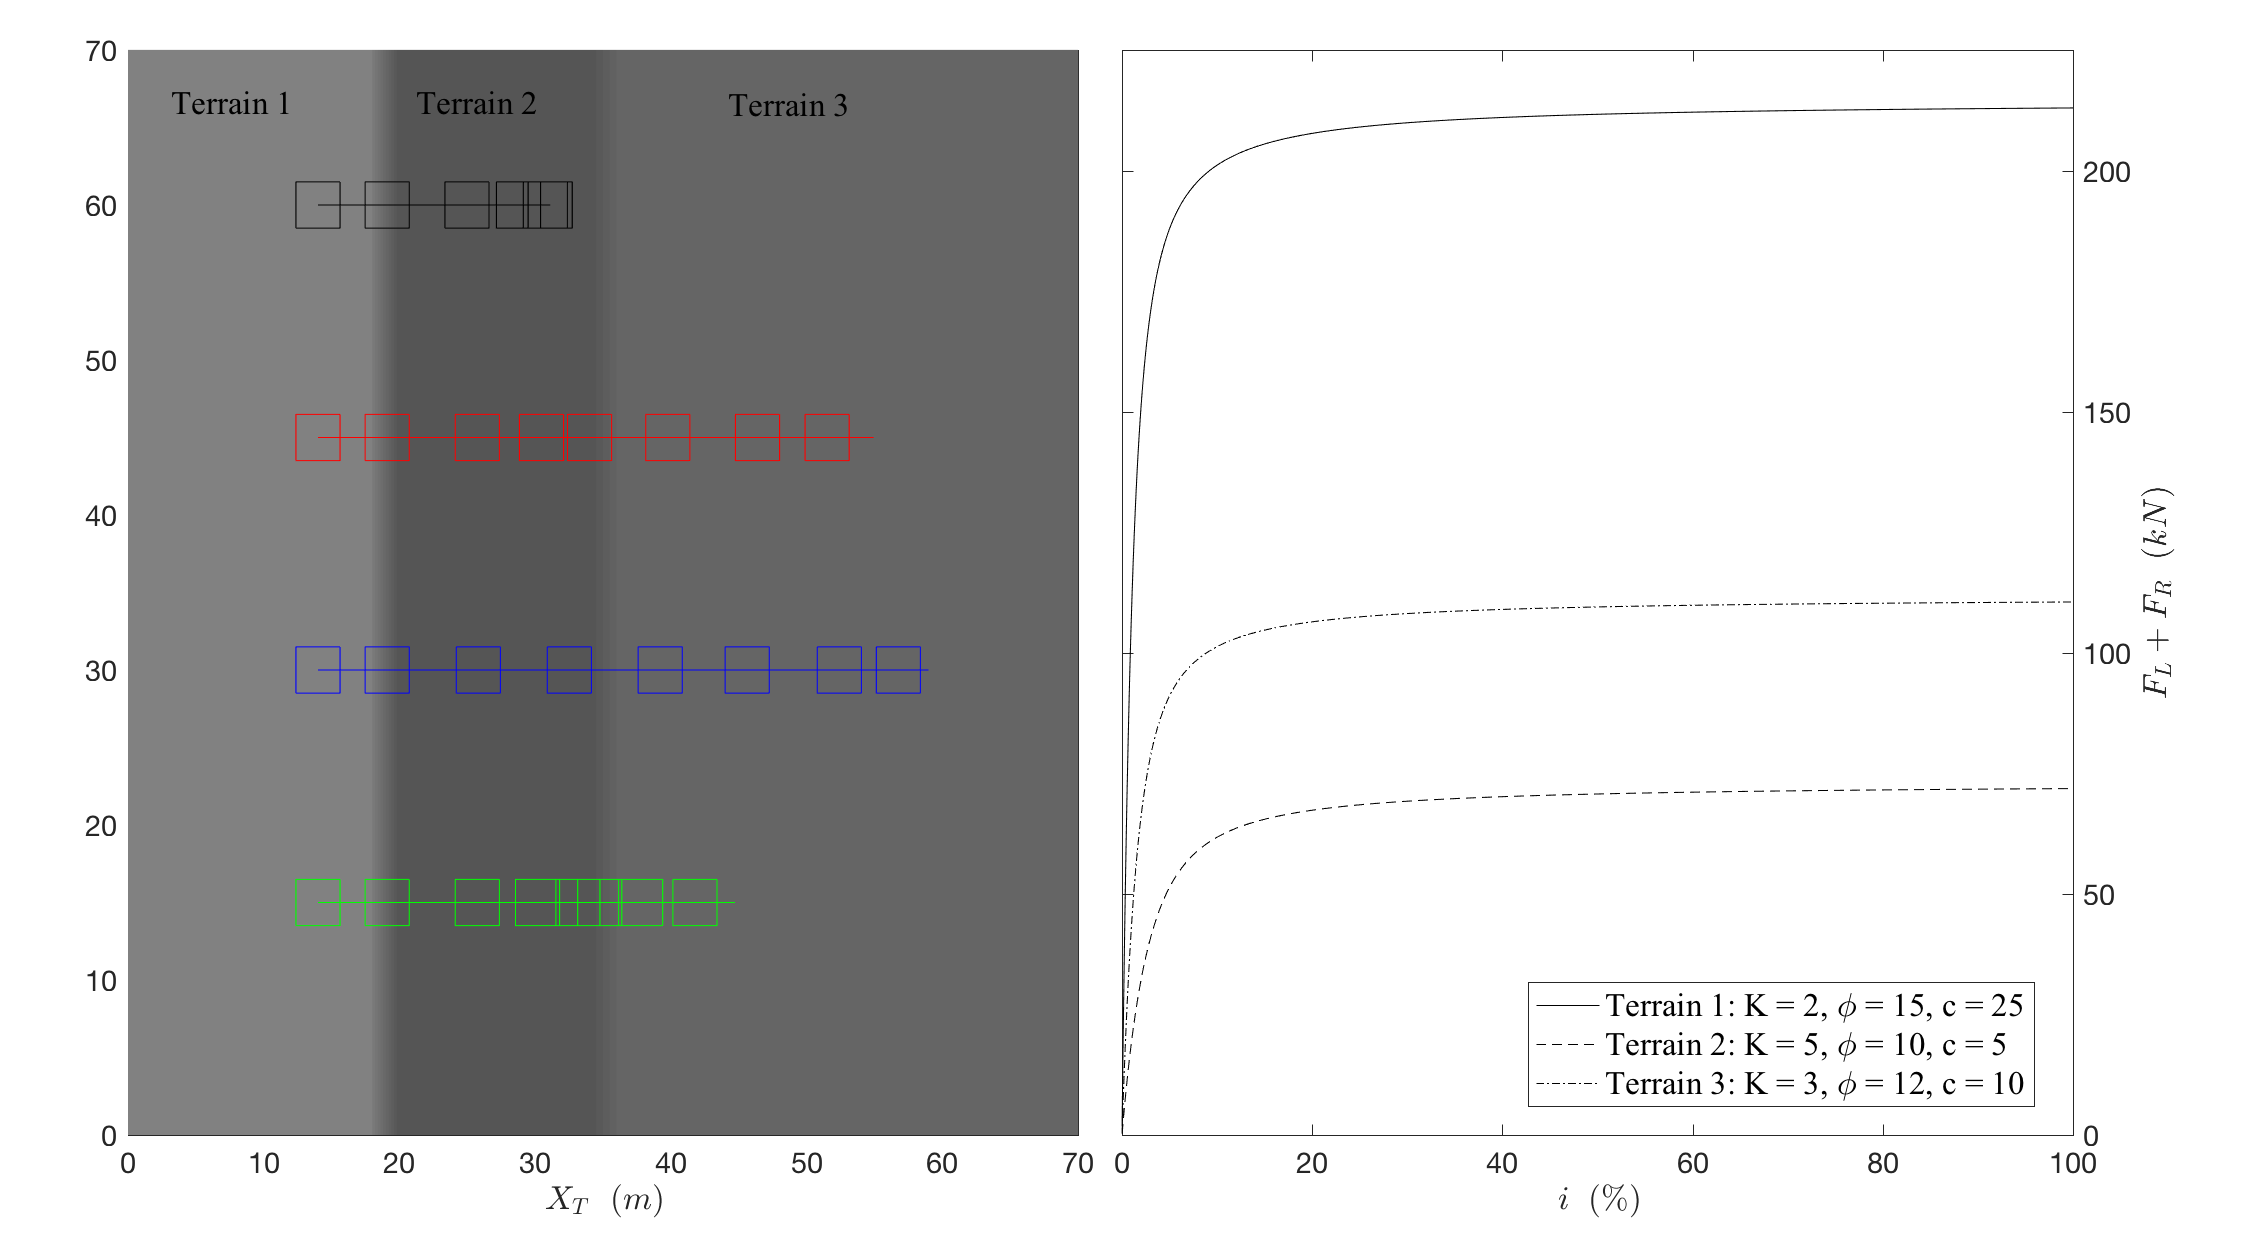
\includegraphics[width = 6in, keepaspectratio]{2D_Plot_4Tractor_MB}
    \caption{Plots of the black, red, blue and green vehicle progress across three terrain zones with force-slip curves defining the available traction forces for each zone. All vehicles are towing an 80,000 kg payload}
    \label{fig:2D_Plot_4Tractor_MB}
\end{figure}
\begin{figure}[ht]
    \centering
    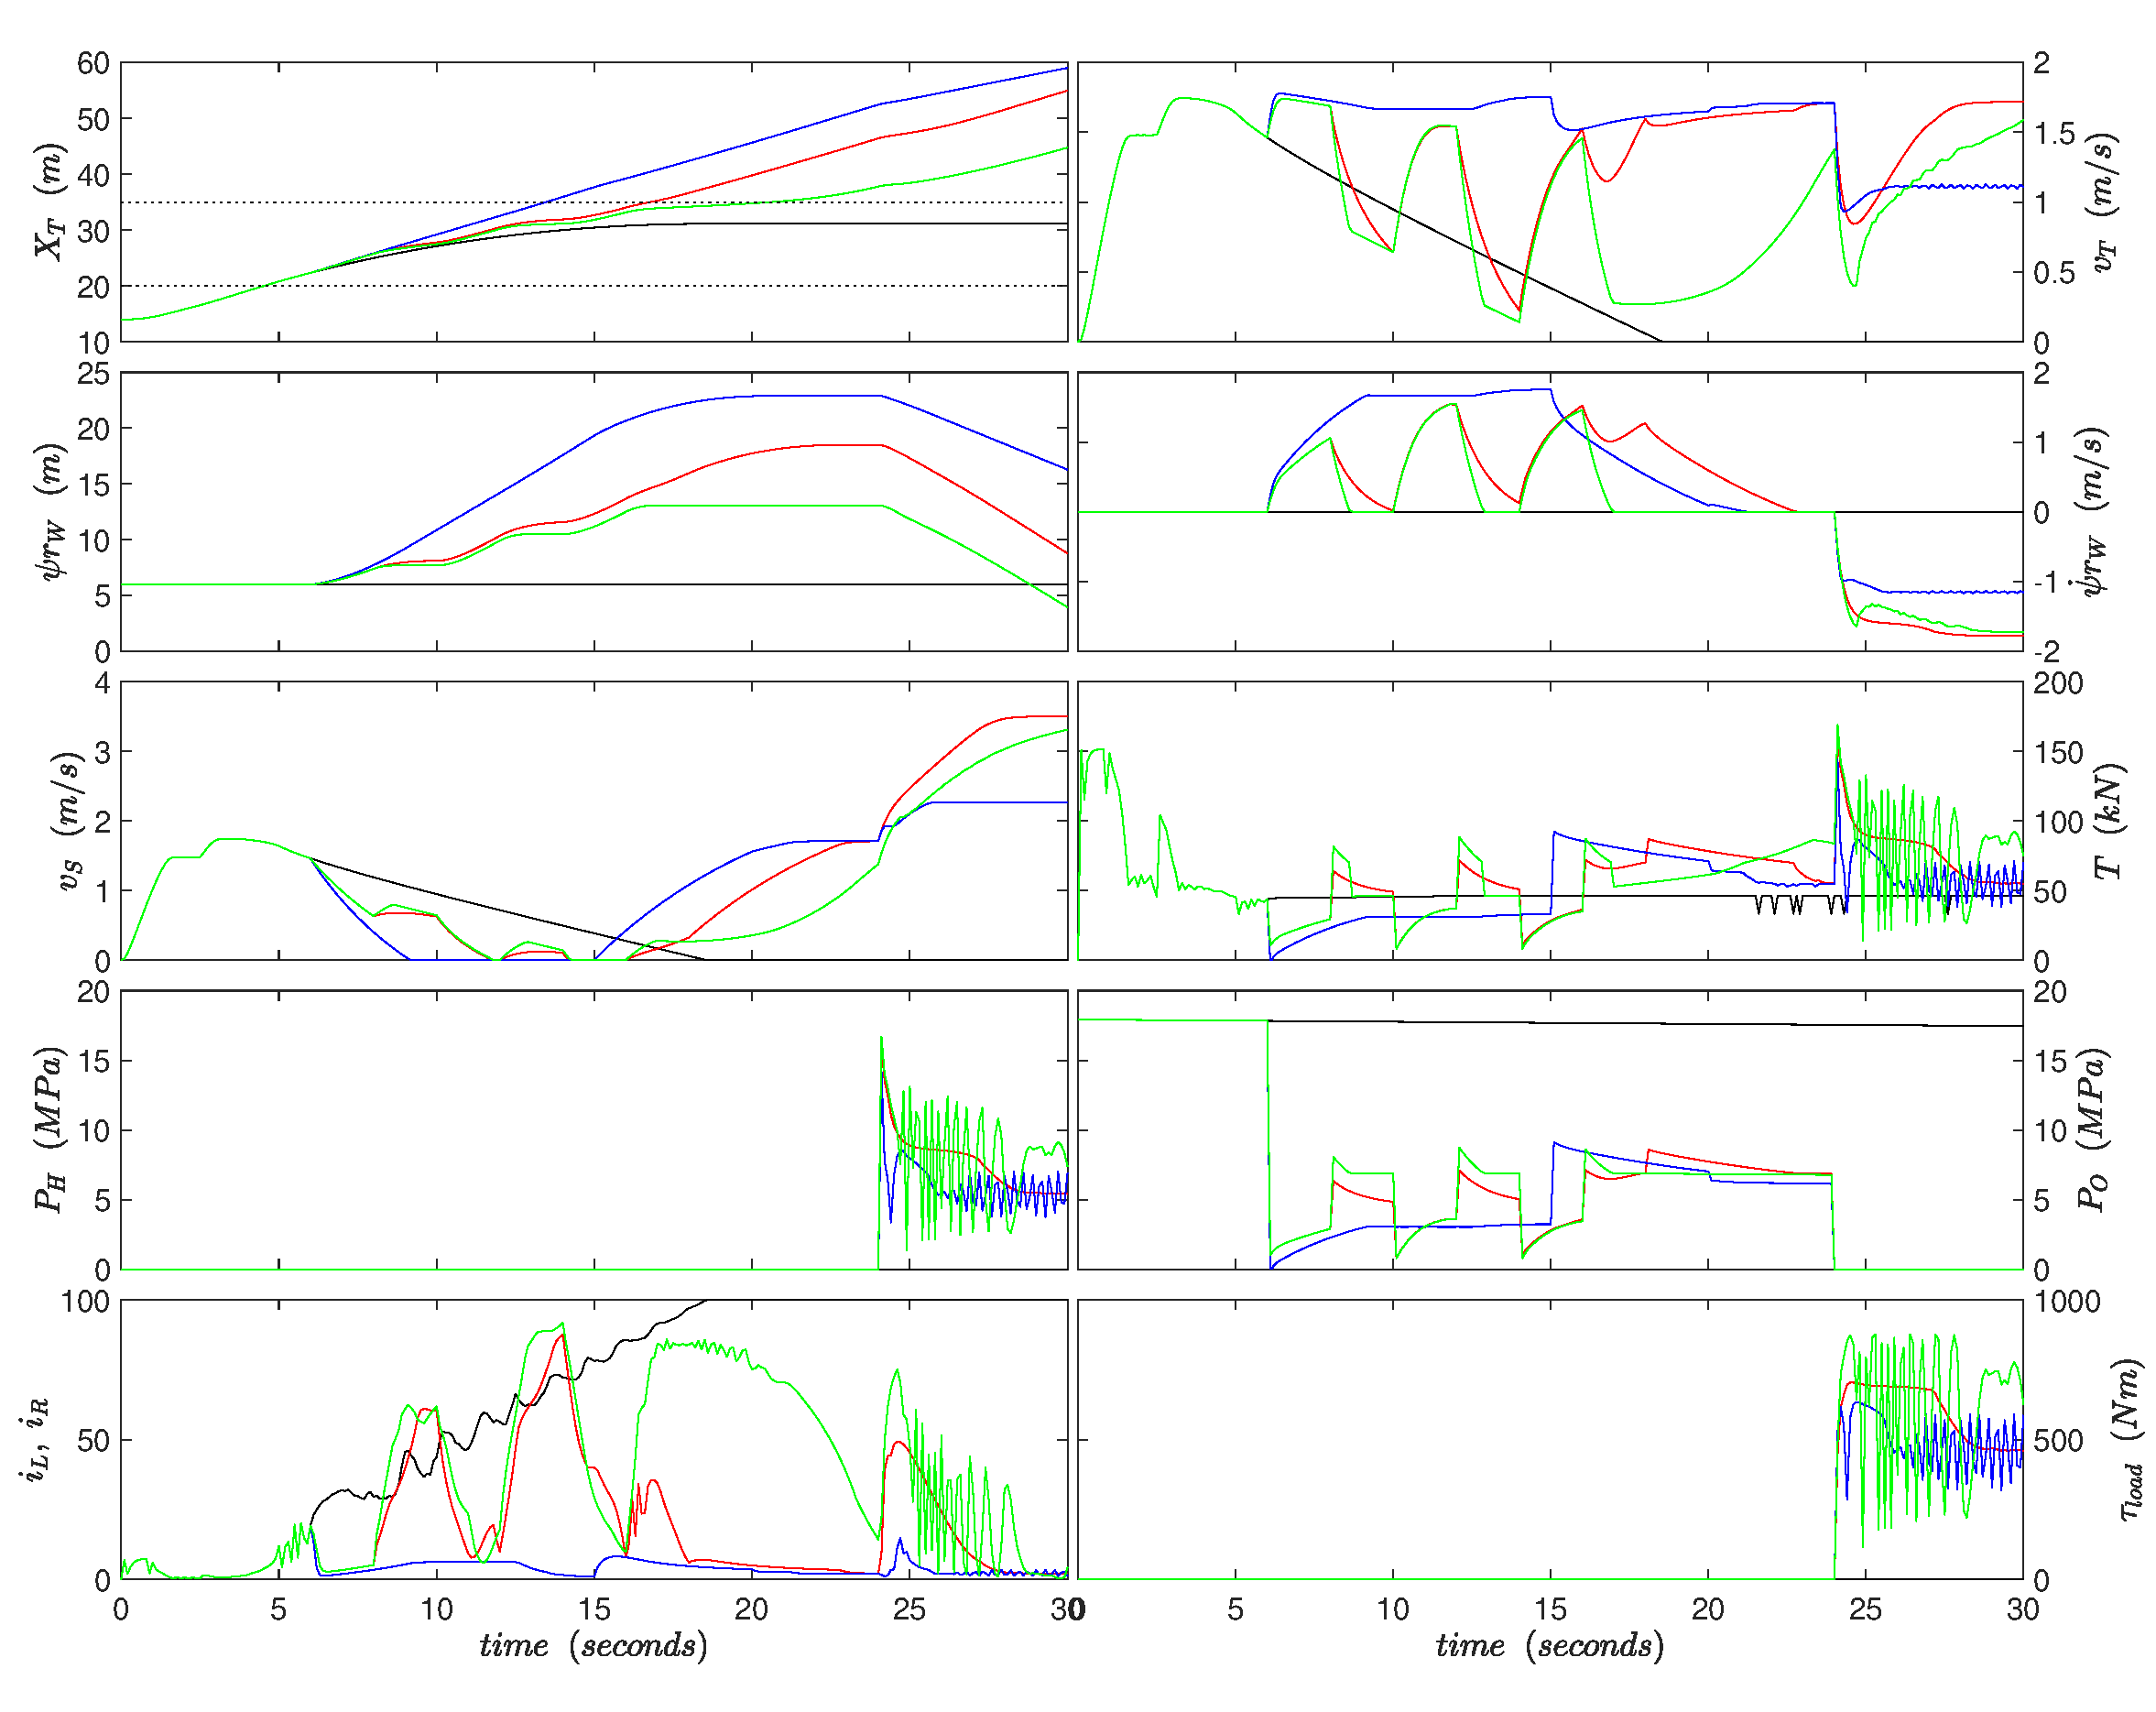
\includegraphics[width = 6in, height = 5.5in]{Traj_4Tractor_MB}
    \caption{Simulation results for the multi-body dynamics model of a tractor-winch-sled system using different sets of open loop control inputs. Colors for all plots correspond to each of four vehicles. All vehicles are towing an 80,000 kg payload}
    \label{fig:Traj_4Tractor_MB}
\end{figure}
is set to close to $P_{Max}$ for an attempt to pull in the towed load too aggressively. In addition, trade offs between the trajectories of the blue and red vehicle can be seen by differences in slip and the rate of cable recovery in Fig. \ref{fig:Traj_4Tractor_MB}.

These simulation results highlight the ability to utilize the winch to maintain mobility while also showing limitations in its abilities for control development. The open-loop pulse breaking strategy used by the red and green vehicles attempts to minimize lost cable length but is unlikely to be viable in practice for two reasons. First, this braking technique impulsively increases the drawbar load at the vehicle induces large track slip values. So far, no slip-sinkage effects are included in the model and it is likely that the slip ratios seen in the red and green tractors trajectory would excavate the vehicle into the terrain and cause immobilzation. Second, there are unmodeled higher frequency cable dynamics that could cause the model to be inaccurate under an impulsive drawbar load that could create undesirable trajectories not seen in simulations. 

The development of the model in this chapter has allowed the use of open-loop inputs to explore possible viable control strategies for the winch control mode via simulation. For automated tractors equipped with towing winches, the control laws developed will focus on producing trajectories similar to the blue vehicle. This conservative approach will aim to be robust across the terrain parameter space and different lengths of soft terrain.  


